\documentclass[letterpaper]{article} % DO NOT CHANGE THIS
\usepackage[submission]{aaai2027} % DO NOT CHANGE THIS
\usepackage[hyphens]{url} % DO NOT CHANGE THIS
\usepackage{graphicx} % DO NOT CHANGE THIS
\urlstyle{rm} % DO NOT CHANGE THIS
\def\UrlFont{\rm} % DO NOT CHANGE THIS
\usepackage{natbib} % DO NOT CHANGE THIS AND DO NOT ADD OPTIONS
\usepackage{caption} % DO NOT CHANGE THIS AND DO NOT ADD OPTIONS
\frenchspacing % DO NOT CHANGE THIS
\usepackage{booktabs}
\usepackage{path}

\pdfinfo{
/TemplateVersion (2027.1)
}

\setcounter{secnumdepth}{1}

\title{Adversarial Course-of-Action Generation: Game-Theoretic Multi-Agent Algorithms for MEF \& GBC}
\author{Anonymous Submission}
\affiliations{}

\begin{document}

\maketitle

\begin{abstract}
Military course-of-action (COA) generation is a recurring planning task in which a force must propose, compare, and select among candidate plans under an adversarial response. We present COA-Bench, a small, fully offline, reproducible framework for studying COA generation policies under self-play, and we formalize its two central scoring quantities under the vocabulary of the Transformational Model for Decision Advantage (TM-DA), an operational battle-management framework in which \emph{Match Effectors} (MEF) pairs a required effect with candidate assets and \emph{Generate BattleCOA} (GBC) assembles matched effectors into an evaluable plan. COA-Bench's MEF and GBC are coarse, scalar analogues of these two DecisionFunctions -- a per-COA effectiveness/cost/risk score and a pairwise force-advantage score, respectively -- reused without modification from the existing \texttt{coageneration} library; this paper introduces no new scoring algorithm and no new mathematics for either quantity. We represent a COA as a typed, chainable sequence of actions with an associated MEF score, evaluate pairs of opposing COAs with a GBC score and Nash-gap distance, and score doctrinal coherence with a heuristic FM 3-0-inspired rubric. Across 90 synthetic scenarios spanning three operational templates (urban stability, maritime interdiction, multi-domain combat), we compare three RED response policies: single random response, sampled best-of-8, and an LLM-backed policy (Claude, \path{claude-haiku-4-5-20251001}). Sampled best-response produces measurably stronger RED COAs by MEF score, lowering BLUE's wargame win rate from 0.900 to 0.811. The LLM policy produces the highest doctrinal alignment of any RED policy (0.804, approaching BLUE's 0.847) but the lowest MEF effectiveness -- BLUE wins \emph{more} against LLM RED (0.911) than against random single-sample RED (0.900) -- revealing that the FM 3-0 rubric and MEF score measure partially distinct properties. We further show that the benchmark's scenario-framing parameter, originally stored as metadata only, had no measurable effect on generated COA content; we trace and repair this gap, reporting a deterministic, honestly-scoped framing-sensitivity effect. All metrics, scenarios, and policies are reused without modification from \texttt{coageneration}; the paper's new artifacts are the experiment script, the framing wiring, an explicit MEF/GBC-to-TM-DA terminology correspondence with its architectural limits stated, and this writeup. Given the moderate scenario count (N=90) and an unvalidated heuristic rubric, these are preliminary, falsifiable findings and a methods contribution, not evidence about real-world COA quality or TM-DA conformance.
\end{abstract}

% Identifying code and artifact links are intentionally omitted for anonymous review.

\section{Introduction}

Course-of-action development is a core step in military operational planning: a staff proposes one or more candidate COAs, wargames each against likely adversary responses, and selects a COA to refine and execute. Two properties of this task make it attractive for studying AI-assisted plan generation. First, COA quality is inherently adversarial -- a COA's effectiveness depends on the opposing force's response, not on a fixed environment. Second, COA quality is doctrinally constrained -- a plan can score well on a narrow effectiveness measure while violating combined-arms balance, sustainment, or risk-mitigation norms that human planners are trained to apply.

Prior agent-evaluation work establishes the value of self-play for discovering strong policies in adversarial games \citep{silver2018alphazero,vinyals2019alphastar,brown2019superhuman}, and more recently in games combining strategic reasoning with natural-language negotiation \citep{bakhtin2022cicero}. Separately, LLM agent benchmarks emphasize interleaving reasoning and action \citep{yao2023react} and evaluating agents end to end rather than on isolated completions \citep{liu2024agentbench}. COA-Bench sits at this intersection: it represents COAs as typed, chainable action sequences (so they can be produced by either a programmatic policy or an LLM-backed one), evaluates them through self-play against an opposing force, and scores them against both a quantitative effectiveness measure and a heuristic doctrinal rubric drawn from U.S. Army FM 3-0 \citep{fm30}.

A separate, operationally oriented line of work names this same conceptual territory differently. The Transformational Model for Decision Advantage (TM-DA) \citep{tmda2025bootcamp} decomposes battle management into precisely defined DecisionFunctions, two of which are named \emph{Match Effectors} (MEF) and \emph{Generate BattleCOA} (GBC): MEF pairs a needed BattleEffect with candidate Effectors, and GBC assembles the resulting matches into a hypergraph of BattleEvents representing one or more complete, evaluable BattleCOAPaths. COA-Bench independently uses the acronyms MEF and GBC for a per-COA effectiveness score and a pairwise force-comparison score. This paper is, in part, an exercise in stating that correspondence precisely: where the two usages align conceptually, and where COA-Bench's scalar scores fall well short of TM-DA's structured, graph-based DecisionFunctions. We treat this as a terminology contribution, not a claim that COA-Bench implements or validates TM-DA.

This paper does not introduce a new benchmark from scratch, nor a new scoring algorithm. The \texttt{coageneration} library already implements the typed COA representation, a self-play engine, a sampled best-response policy, bootstrap confidence intervals, a multi-COA comparison utility, an FM 3-0-inspired doctrinal rubric, and a stylized Lanchester-attrition wargame check, all built around the existing MEF and GBC formulas. Our contributions are:
\begin{itemize}
  \item a precise, explicitly bounded correspondence between COA-Bench's MEF/GBC scores and TM-DA's Match Effectors / Generate BattleCOA DecisionFunctions, stating both the analogy and its limits (Section~\ref{sec:tmda});
  \item a single coherent 90-scenario self-play experiment exercising the existing \texttt{coageneration} machinery, rather than isolated unit tests;
  \item a comparison of three RED response policies (single-sample, sampled best-of-8, LLM-backed) on MEF/GBC, doctrinal alignment, Nash-gap, and wargame outcome; and
  \item a documented methodological gap -- a scenario-framing parameter that silently had no effect on generated content -- traced, fixed, and reported honestly rather than omitted.
\end{itemize}

Concretely, we ask three questions: (1)~does sampling several candidate best-responses and keeping the best one change the responding force's GBC score, doctrinal alignment, and wargame win rate relative to generating a single response? (2)~does an LLM-backed COA policy (Claude) produce stronger RED responses than random sampling by any of these metrics? (3)~does the benchmark's scenario-framing parameter actually change generated COA content, and if so, by how much? We report measured answers to all three over 90 scenarios (30 seeds $\times$ 3 operational templates), with bootstrap 95\% confidence intervals throughout. The implementation, experiment script, and raw results are available at \texttt{experiments/coa\_bench\_experiment.py} and \path{results/coa-bench/main/} in the accompanying repository.

\section{Related Work}

\paragraph{Self-play and adversarial game evaluation.} Prior work establishes self-play as a method for discovering strong policies in adversarial games with large action spaces, without requiring human-labeled examples of optimal play \citep{silver2018alphazero,vinyals2019alphastar,brown2019superhuman}. CICERO extends self-play to a game requiring natural-language negotiation alongside strategic planning \citep{bakhtin2022cicero}. COA-Bench borrows the self-play structure -- a policy responds to an opposing force's COA, and the pair is scored jointly -- but operates over a much smaller, synthetic action space and does not (yet) train a policy from self-play; the current policies are a random sampler and an LLM-backed generator, evaluated rather than trained.

\paragraph{Strategic and military decision modeling.} Lanchester's combat-attrition equations \citep{lanchester1916} and Schelling's game-theoretic treatment of strategic conflict \citep{schelling1960} are foundational, non-learned models of adversarial military interaction; COA-Bench's wargame check is a deliberately simplified, score-linked variant of a Lanchester model, used as a secondary outcome measure rather than a validated combat model. FM 3-0 \citep{fm30} specifies qualitative planning criteria (objective clarity, combined-arms balance, sustainment, risk mitigation, tempo) that COA-Bench's rubric operationalizes heuristically; the rubric is a benchmark feature extractor, not a substitute for doctrine-expert validation.

\paragraph{Battle-management decision functions (TM-DA).} TM-DA \citep{tmda2025bootcamp} models battle management as a sequence of DecisionFunctions operating over hypergraphs of typed BattleEvents. Match Effectors (MEF) searches for and ranks candidate Effectors against a needed BattleEffect, producing EffectEffectorMatches; Generate BattleCOA (GBC) then weaves those matches -- together with resourcing, temporal, and mutual-exclusion constraints -- into one or more physically possible, tactically valid BattleCOAPaths, which a battle manager compares before sequencing. This is substantially richer than a scalar score: TM-DA's GBC output is a hypergraph of alternatives, evaluated against explicit criteria (physical possibility, tactical soundness, parsimony, worldline completeness, adjudicated consequences), not a single number. COA-Bench's MEF score (Section~\ref{sec:tmda}) is a coarse analogue of how well a COA's chosen actions trade off effectiveness against cost and risk -- the same intuition MEF is meant to capture, computed very differently -- and its GBC score is a coarse analogue of comparing two candidate plans, without representing assembly, worldlines, or multi-path hypergraphs. We adopt the acronyms for readability and conceptual continuity, not as a claim of architectural or numerical equivalence.

\paragraph{LLM agent and planning evaluation.} ReAct interleaves reasoning and acting in language-model agents \citep{yao2023react}, and AgentBench evaluates LLM agents end to end across interactive environments rather than on isolated completions \citep{liu2024agentbench}. COA-Bench's typed action/chain representation, including conditional branches and tool calls, is designed so the same evaluation pipeline can score both a programmatic sampling policy and an LLM-backed policy; this paper evaluates all three under the same protocol.

\paragraph{COA generation and computational military planning.} Automated course-of-action generation has been studied using knowledge-based planners, simulation-driven evaluation, and agent-based modeling \citep{sokolowski2010military}. The U.S. Military Decision Making Process (MDMP), codified in JP 5-0 \citep{jp50}, defines a seven-step planning cycle in which COA development, wargaming, and comparison are sequential staff functions; COA-Bench operationalizes the comparison and wargaming steps in a lightweight, reproducible form. Cummings \citep{cummings2017artificial} surveys the longer-term implications of AI for military decision-making, highlighting the challenge of integrating automated systems into human staff processes without eroding human accountability. The companion framework from the same repository, MetaRoute-Bench \citep{vidra2026metaroute}, applies a similar benchmark-design philosophy to LLM routing policy evaluation; a practical lesson from COA-Bench's framing bug (Section~\ref{sec:framing}) is cited in that work's own practical-lessons discussion.

\section{Problem Formulation and MEF/GBC Correspondence}
\label{sec:tmda}

A COA is a typed object: an ordered or chained set of Actions (each with a category, target, priority, and optional tool call), an optional conditional branch, an objective string, a force assignment (BLUE or RED), a domain tag, and a scalar MEF score. Formally,
\begin{equation}
\mathrm{MEF} = \mathrm{clamp}_{[-1,1]}\big(w_e \cdot e - w_c \cdot c - w_r \cdot r\big),
\end{equation}
where $e$, $c$, and $r$ are a COA's effectiveness, cost, and risk components and default weights are $w_e=0.5$, $w_c=0.3$, $w_r=0.2$. Two opposing COAs are compared with
\begin{equation}
\mathrm{GBC} = \frac{\mathrm{MEF}_{\mathrm{blue}} - \mathrm{MEF}_{\mathrm{red}} + 2}{4} \in [0,1],
\end{equation}
and with a Nash-gap distance $|\,\mathrm{payoff}_{\mathrm{blue}} + \mathrm{payoff}_{\mathrm{red}} - 1\,|$ after MEF scores are rescaled to $[0,1]$ payoffs. Both formulas are unmodified from the pre-existing \texttt{coageneration} library (\texttt{compute\_mef\_score}, \texttt{gbc\_score}); this paper changes neither.

TM-DA \citep{tmda2025bootcamp} independently defines MEF (\emph{Match Effectors}) and GBC (\emph{Generate BattleCOA}) as sequential DecisionFunctions rather than scalar scores. Table~\ref{tab:correspondence} states the correspondence we draw between the two usages, and its limits.

\begin{table}[t]
\centering
\small
\caption{Correspondence between COA-Bench's MEF/GBC scores and TM-DA's MEF/GBC DecisionFunctions. COA-Bench implements the scalar column only.}
\label{tab:correspondence}
\begin{tabular}{p{0.11\linewidth}p{0.37\linewidth}p{0.37\linewidth}}
\toprule
 & TM-DA DecisionFunction & COA-Bench scalar (this paper) \\
\midrule
MEF & Searches for and ranks candidate Effectors against a needed BattleEffect; output is a ranked set of EffectEffectorMatches. & A single number per COA trading off effectiveness against cost and risk; no explicit asset-search or ranking step. \\
\addlinespace
GBC & Assembles matched Effectors, with resourcing/temporal/mutual-exclusion constraints, into a hypergraph of one or more complete BattleCOAPaths; output is compared alternatives, not one number. & A single number in $[0,1]$ expressing one force's MEF advantage over an opposing force's fixed COA; no path assembly, worldlines, or multi-path hypergraph. \\
\bottomrule
\end{tabular}
\end{table}

We use TM-DA's names because both pairs describe the same two conceptual moments in COA generation -- matching a plan's constituent choices to the effect they should produce, and generating/comparing complete candidate plans -- but COA-Bench's scores are coarse, single-scalar simplifications, not implementations of TM-DA's DecisionFunctions. A reader who expects TM-DA-conformant hypergraph outputs, worldline-completeness checking, or EffectEffectorMatch ranking from this paper's MEF or GBC will not find them here; extending \texttt{coageneration} toward that richer representation is future work (Section~\ref{sec:limitations}).

Given an opposing force's COA, a policy generates a response for the same scenario's \texttt{GameState}. The baseline policy draws one random response (\texttt{SelfPlayEngine.best\_response}). \texttt{SampledBestResponsePolicy} draws $n$ candidate responses and either returns the single highest-MEF candidate or exposes all $n$ candidates for downstream comparison. \texttt{compare\_coas} ranks a candidate set by MEF, computes heuristic doctrinal alignment per candidate, measures action-type diversity (mean pairwise Jaccard distance), and identifies the Pareto-optimal subset on (MEF, doctrinal alignment) -- the closest COA-Bench analogue to TM-DA's presentation of multiple BattleCOAPaths for a battle manager's review, though over a flat candidate list rather than a path hypergraph.

\texttt{fm30\_rubric\_scores} extracts six heuristic, doctrine-inspired terms -- objective clarity, intelligence preparation, combined-arms balance, sustainment, risk mitigation, and tempo/sequencing -- each in $[0,1]$, from a COA's objective text and action categories; \texttt{doctrinal\_alignment\_score} is their weighted aggregate. \texttt{lanchester\_wargame\_outcome} runs a stylized multi-step attrition simulation in which each side's effective combat power is scaled by $1 + \mathrm{MEF} + \mathrm{doctrinal\_alignment}$, so COA quality directly affects the wargame outcome and not only the COA-level metrics.

Three factory functions generate operational templates -- urban stability operations, maritime interdiction, and multi-domain large-scale combat -- each parameterized by a random seed and a \texttt{framing} string (\texttt{"blue"}, \texttt{"neutral"}, or \texttt{"adversary"}) representing how a scenario is narratively framed to the planner.

\section{Experimental Protocol}

We generate 90 scenarios: 30 base seeds $\times$ 3 operational templates (urban, maritime, multi-domain). For each scenario we fix the first seed COA as BLUE and generate a RED response three ways: (a) single random best-response, (b) sampled best-response over $n=8$ candidates, and (c) an LLM-backed response (\texttt{LLMPolicy} using \path{claude-haiku-4-5-20251001} via the Anthropic API). We compute GBC and Nash-gap for all three RED variants against the same BLUE COA, doctrinal alignment for BLUE and all three RED variants, a multi-COA comparison over the 8 sampled candidates, and a Lanchester wargame outcome for BLUE against each RED variant. All confidence intervals are 95\% percentile-bootstrap intervals over the 90 scenarios (1{,}000 resamples). No held-out or challenge split is used: this is a single fixed synthetic scenario set, and we do not claim generalization beyond it.

\section{Results}

\subsection{Main Comparison: Sampling Policies}

\begin{table}[t]
\centering
\small
\caption{RED policy comparison over 90 scenarios. CI is the 95\% bootstrap interval. LLM policy uses Claude (\path{claude-haiku-4-5-20251001}).}
\label{tab:main}
\begin{tabular}{lrrr}
\toprule
Metric & Single & Sampled ($n{=}8$) & LLM \\
\midrule
GBC (blue adv.) & .524 [.519,.530] & .490 [.487,.494] & .549 [.546,.552] \\
Nash gap & .199 [.189,.209] & .267 [.261,.274] & .150 [.143,.157] \\
Red doct. align. & .667 [.640,.695] & .678 [.658,.700] & .804 [.780,.831] \\
Blue win rate & .900 & .811 & .911 \\
\bottomrule
\end{tabular}
\end{table}

\begin{figure}[t]
\centering
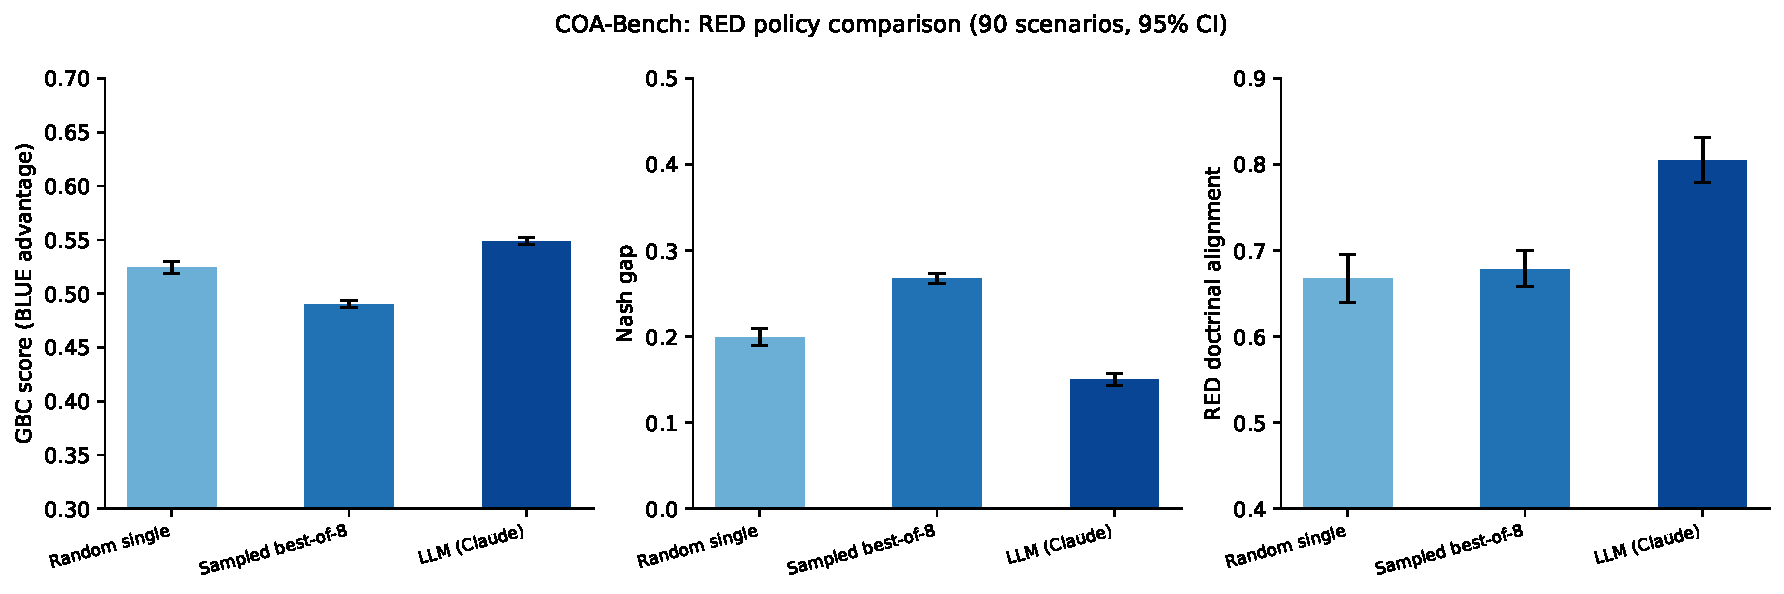
\includegraphics[width=\linewidth]{figures/policy_comparison.pdf}
\caption{GBC score, Nash gap, and RED doctrinal alignment for single-sample, sampled ($n{=}8$), and LLM (Claude) RED policies across 90 scenarios. Error bars are 95\% bootstrap CIs.}
\label{fig:policy}
\end{figure}

Table~\ref{tab:main} and Figure~\ref{fig:policy} report all three RED policies. Letting RED sample 8 candidate responses and keep its best-MEF one makes RED a measurably tougher opponent: GBC falls from .524 to .490 because RED's MEF rises under best-of-8 selection, and the Nash-gap distance from equilibrium grows (.199 to .267) because RED's payoff increases without a corresponding adjustment to BLUE's fixed COA. BLUE's wargame win rate falls from .900 to .811 -- an independent confirmation via a different mechanism (attrition simulation rather than MEF scores directly). RED's doctrinal alignment is \emph{higher} under best-of-8 selection (.678 vs.\ .667): in this synthetic action space, selecting for MEF did not cost doctrinal coherence.

\subsection{LLM Policy: Doctrinal Coherence Without MEF Effectiveness}

The LLM RED policy produces a qualitatively different profile from either sampling baseline. Its doctrinal alignment (.804) substantially exceeds both single-sample (.667) and sampled best-of-8 (.678), approaching BLUE's own alignment (.847). The prompt instructs Claude to generate a ``strategic counter-COA'' as a typed JSON object with an objective and 2--5 actions, so it naturally produces plans that read like well-structured doctrine -- covering multiple categories, stating clear objectives -- which is precisely what the FM 3-0 rubric rewards.

LLM RED's MEF effectiveness is nonetheless the weakest of the three policies: BLUE's GBC score against it (.549) exceeds GBC against random single-sample RED (.524), and BLUE's wargame win rate against LLM RED (.911) exceeds both sampling baselines (.900, .811). The LLM optimizes for plan coherence as it interprets the prompt, not for the \texttt{mef\_score} field \texttt{SampledBestResponsePolicy} explicitly maximizes. Because MEF score is what actually drives wargame outcomes in this simulator, doctrinal coherence and strategic effectiveness are partially decoupled: the LLM wins the rubric comparison but loses the attrition simulation. The Nash gap for LLM RED (.150) is the smallest of the three, not because the LLM found a strong equilibrium response, but because its lower MEF pulls the payoff split toward the center.

Under the TM-DA correspondence of Section~\ref{sec:tmda}, this is a concrete illustration of why MEF and doctrinal review are meant to be distinct checks: a plan (or EffectEffectorMatch) that reads as well-formed is not automatically one that has been ranked highly against the effect it is meant to produce. We treat the pattern -- high rubric score, low MEF, small Nash gap -- as a benchmark diagnostic revealing that the FM 3-0 rubric and MEF measure different properties of a COA.

\subsection{Route Quality: Multi-COA Comparison}

Applying \texttt{compare\_coas} to the 8 sampled RED candidates per scenario gives a mean candidate diversity (mean pairwise Jaccard distance of action types) of .732 [.720,.745], a mean MEF spread of .254 [.245,.264], and a mean of 2.15 [1.978,2.333] Pareto-optimal candidates out of 8 on the (MEF, doctrinal alignment) frontier. Roughly a quarter of the 8 sampled candidates are simultaneously non-dominated on effectiveness and doctrinal alignment, indicating the candidate set is not redundant and motivating human review of the Pareto-optimal subset rather than a single auto-selected candidate. Figure~\ref{fig:pareto} shows the (MEF, doctrinal alignment) scatter for the first 10 scenarios.

\begin{figure}[t]
\centering
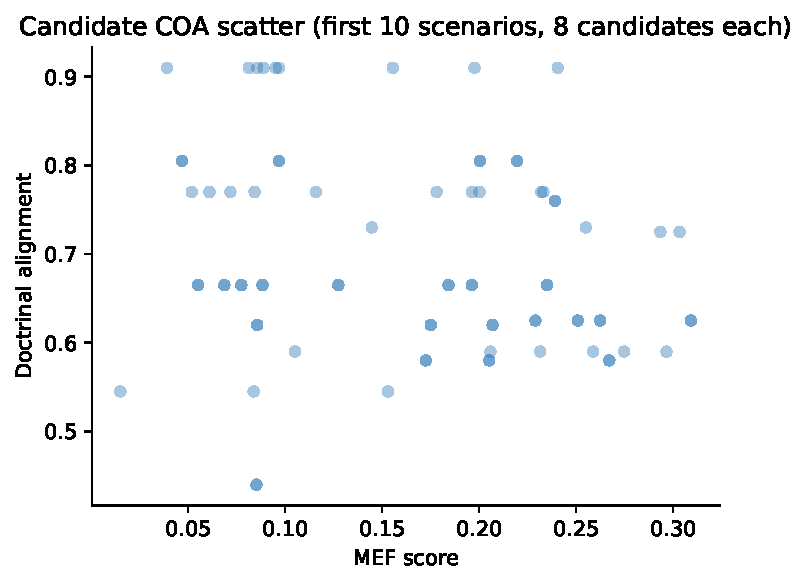
\includegraphics[width=\linewidth]{figures/pareto_scatter.pdf}
\caption{MEF score vs.\ doctrinal alignment for $8 \times 10$ sampled RED candidates (first 10 scenarios). There is no single dominant corner, motivating human review of the Pareto-optimal subset.}
\label{fig:pareto}
\end{figure}

\subsection{Sensitivity: The Scenario-Framing Repair}
\label{sec:framing}

While building this experiment we found that \path{ScenarioProfile.framing} -- intended to represent how a scenario is narratively framed to the planner (favorable to BLUE, neutral, or favorable to the adversary) -- was stored as scenario metadata only and never affected generated COA content. A naive framing-sensitivity ablation (\texttt{doctrinal\_alignment\_score} of the same seed COA under three framing labels) returned an exact 0.0 delta with zero variance across all 30 scenario-seeds: a measurement of a no-op, not evidence that framing has no effect.

We traced this to two compounding causes: (1) the factory functions accepted a \texttt{framing} argument but never used it in the objective string or action list, and (2) even after wiring framing into the objective text, several FM 3-0 rubric terms (risk mitigation, objective clarity) were already saturated at 1.0 by fixed, framing-independent scenario content -- e.g., the urban template's branch unconditionally includes a \texttt{withdraw} action and the maritime template unconditionally includes a \texttt{compliant\_boarding} action, both of which trigger the risk-mitigation term regardless of framing. We fixed this by (a) making framing change the primary COA's objective text and (b) having \texttt{"blue"} framing append one additional action in a category the COA does not already use, moving the \texttt{combined\_arms\_balance} term -- the one dimension with headroom in all three templates. After this fix, \texttt{framing\_sensitivity\_delta} returns .045 [.045,.045] across all 30 scenarios.

We report the zero-width interval as-is: the .045 delta is currently a deterministic function of the framing label, not a sampled effect with scenario-to-scenario variance, because our fix adds exactly one fixed action under exactly one framing condition. This is real progress over the prior no-op and a concrete target for replacing the deterministic rule with a richer, sampled framing-conditioned generator.

\section{Discussion}

\subsection{Interpretation}

Three conclusions follow within this benchmark. First, sampled best-response is a strictly stronger RED policy than single-sample by every MEF-linked metric (GBC, Nash-gap, wargame win rate), and this strength does not come at the cost of doctrinal alignment in this action space. Second, an LLM-backed policy optimizing implicitly for plan coherence under a natural-language prompt is not the same as a policy optimizing explicitly for MEF, and the two can diverge sharply: the LLM is the most doctrinally aligned RED policy and simultaneously the weakest by strategic effectiveness. Third, a benchmark parameter that is stored as metadata but not wired into content generation produces a silent measurement no-op rather than a true null result -- a general lesson, not specific to COA-Bench, that also surfaced independently in the companion MetaRoute-Bench study \citep{vidra2026metaroute}.

\subsection{MEF/GBC Terminology: What Carries Over and What Does Not}

The TM-DA correspondence in Table~\ref{tab:correspondence} is useful for readers already fluent in battle-management DecisionFunction vocabulary, but it should not be over-read. COA-Bench's MEF is a single number; it does not search a space of candidate assets or produce ranked EffectEffectorMatches. COA-Bench's GBC is a single comparison score; it does not assemble a hypergraph of BattleCOAPaths, check worldline completeness, or adjudicate mutual exclusions between assets. The LLM-policy result in Section~4.2 is, if anything, a demonstration of why the richer TM-DA process exists: a coherent-looking plan (high rubric score) is not the same as a plan that has been rigorously matched and ranked against the effect it targets (low MEF), and a full Generate BattleCOA process -- rather than a single scalar comparison -- is one way an operational system could catch that gap before it reaches a decision-maker. Closing this gap between COA-Bench's scalar approximation and TM-DA's structured DecisionFunctions is future work, not a claim already established here.

\subsection{Limitations and Threats to Validity}
\label{sec:limitations}

\paragraph{Construct validity.} \texttt{fm30\_rubric\_scores} is a keyword- and category-based feature extractor inspired by FM 3-0 planning criteria, not a substitute for scoring by doctrine experts. The saturation effects documented in Section~\ref{sec:framing} (a single fixed action unconditionally satisfying the risk-mitigation term) show the rubric can be insensitive to genuinely important plan content. Any claim about ``doctrinal alignment'' should be read as ``score under this heuristic rubric.'' Similarly, MEF and GBC should be read as COA-Bench's specific scalar definitions (Section~\ref{sec:tmda}), not as validated measures of real-world plan quality or as implementations of TM-DA's DecisionFunctions.

\paragraph{Internal validity.} The framing fix (Section~\ref{sec:framing}) demonstrates that framing \emph{can} be made to matter, using the smallest change that produces a measurable, non-zero, honestly-reported effect; it is not a claim that real scenario framing in military planning has this specific structure or magnitude of effect. The LLM comparison uses one model (\path{claude-haiku-4-5-20251001}) and one fixed prompt; different models or prompts would likely produce different doctrinal-alignment and MEF profiles, and the coherence-versus-effectiveness decoupling finding is specific to this model--prompt--simulator combination.

\paragraph{External validity.} N=90 scenarios (30 seeds $\times$ 3 templates) comes from three fixed factory functions, not a sampled distribution of real operational situations; the bootstrap confidence intervals quantify sampling variation over this fixed set, not generalization to a broader scenario population. All outcomes come from the offline \texttt{coageneration} simulator; no live planner, real intelligence data, or operational system was used or affected.

\paragraph{Statistical validity.} All reported intervals are 95\% percentile-bootstrap intervals over the 90-scenario set (1{,}000 resamples); they describe sampling variation under this fixed corpus, not an external scenario population. The framing-sensitivity interval is degenerate by construction (Section~\ref{sec:framing}) because the current fix is deterministic, not sampled -- we report this rather than obscuring it.

\section*{Ethical Statement}

COA-Bench operates in a domain -- military operations planning -- where automated systems carry heightened accountability requirements. All scenarios are fictional constructs that do not describe any real operation, location, or force; the benchmark performs no real-world action and contains no personal, classified, or proprietary data. COA-Bench is an evaluation harness, not a planning assistant: it is not connected to any command system and is not intended to support real operational decision-making. Methods for automated adversarial reasoning can, in principle, be adapted for misuse; the action model and scenario space are deliberately kept at an abstracted, synthetic level encoding no operational specifics or intelligence about real targets. The TM-DA document cited for terminology (Section~\ref{sec:tmda}) is an unclassified, distribution-A training briefing describing a conceptual model, not an operational system or targeting data, and is cited here solely for its DecisionFunction naming and definitions. This paper documents two gaps explicitly rather than omitting them: the scenario-framing no-op we found and fixed (Section~\ref{sec:framing}), and the architectural limits of the MEF/GBC-to-TM-DA correspondence we draw (Table~\ref{tab:correspondence}) -- an important norm in military AI research, where overstating evaluation quality or terminology alignment can have real consequences if methods are prematurely deployed or misread as validating an operational framework.

% Acknowledgments are omitted for anonymous review.

\bibliography{references}

\end{document}
